\documentclass{amsart}

\usepackage[title]{appendix}
\usepackage{graphicx}
\usepackage{amsfonts}
\usepackage{url}
\usepackage{amscd}
\usepackage{amssymb}
\newtheorem{algor}{\bf{Algorithm}}[section]
\usepackage[algosection,lined,boxed,commentsnumbered,ruled,vlined]{algorithm2e}
\usepackage[hidelinks]{hyperref}
\newcommand{\todo}[1]
{\marginpar{\baselineskip0ex\rule{2,5cm}{0.5pt}\\[0ex]{\tiny\textsf{#1}}}}

\newtheorem{remark}{Remark}[section]

\newtheorem{theorem}{Theorem}[section]
\newtheorem{lemma}[theorem]{Lemma}	
\newtheorem{corollary}[theorem]{Corollary}
\newtheorem{definition}[theorem]{Definition}
\newtheorem{proposition}[theorem]{Proposition}
%\theoremstyle{remark}
%\newtheorem{example}[theorem]{Example}
%\newtheorem{remark}[theorem]{Remark}
\numberwithin{equation}{section}
\def\L{\mathcal{L}}


%\documentclass[20pt, a4paper]{article}
\usepackage{indentfirst}
\usepackage[greek,english]{babel}
\usepackage[utf8]{inputenc}
\usepackage{color,amsmath,amssymb,graphicx}
\usepackage{tikz-cd}
\usepackage{amsmath,amssymb}
\usepackage{enumerate}
\usepackage{dsfont}
%\usepackage{appendix}
\usepackage{amsthm}
\usepackage{float}
\usepackage[algosection,lined,boxed,commentsnumbered,ruled,vlined]{algorithm2e}
\usepackage{mathtools}
\DeclarePairedDelimiter\floor{\lfloor}{\rfloor}
 	
\begin{document}
	\title[Improved shared secret attacks in NTRU]{Improved shared secret attacks in NTRU and their relation with VFK lattices}
\keywords{Public Key Cryptography; NTRU Cryptosystem; Lattices; LLL algorithm; Closest Vector Problem; Voronoi First Kind;}
\subjclass[2010]{94A60}
%\subjclass[2010]{94A60, 11T71, 11H06, 68R01}
\maketitle	
	\begin{abstract}
		\end{abstract}
\section{Introduction}
The NTRU cryptosystem was created by Hoffstein, Pipher, and Silverman in 1996 as a means of encryption and signature. Its security is based on the difficulty of solving a system of linear equations over polynomial rings, a problem that is expected to remain hard even with quantum computers. While it is not equivalent to the Shortest and Closest Vector Problems (SVP/CVP) in lattices, the NTRU cryptosystem has withstood over 20 years of cryptanalysis and variants of it have been shown to be secure under the Ring Learning With Error (R-LWE) hardness assumption. NTRU is known for its exceptional performance and moderate key-size, making it a popular choice for embedded cryptography. It has been standardized by IEEE, X9.98, PQCRYPTO, and was a finalist in the NIST post-quantum cryptography standardization effort. Ultimately, the Kyber algorithm was selected for standardization. It is also noted in the  3rd Status Report of NIST for PQC\footnote{\url{https://nvlpubs.nist.gov/nistpubs/ir/2022/NIST.IR.8413.pdf}}, the overall performance of any of these KEMs (i.e. Kyber, Saber and NTRU) would be acceptable for general-use applications. Also, NTRU-HRSS was chosen by Google for their ALTS protocol (ALTS:Application Layer Transport Security) in the hybrid model\footnote{\url{https://cloud.google.com/blog/products/identity-security/why-google-now-uses-post-quantum-cryptography-for-internal-comms}}.

\subsection{Relevant work}
The idea to use a lattice attack on the Ntru cryptosystem dates back to 1997, by Coppersmith \cite{CopSha97}.
Furthermore,Gentry discovered a successful strategy that is effective, particularly when N is composite \cite{gentry}.May \cite{May} used a distinct class of lattices, which he named run-lattices, to approach the issue.In \cite{Silverman},Silverman expanded on May's concept and put forth a technique in which he chooses the r coefficients and forces them to equal zero by reducing the dimension of the lattice.In \cite{Gama-Nguyen},the authors make use of decryption failures.In reality, the secret key may be recovered if one has access to an NTRUencrypt decryption oracle with a parameter set that permits decryption failures.In \cite{witt} and furthermore in \cite{gerald},the authors reduced the NTRU issue to a multivariate quadratic system over the Galois field with two elements using Witt vectors.
In \cite{Odlyzko},the authors described the attack by Andrew Odlyzko, which is a meet-in-the-middle attack.In order to find the secret key, they divided the search area into two parts and utilized a collision search technique.The time complexity is therefore reduced. Its disadvantage is the high memory requirement.The hybrid attack that Howgrave presents is an intriguing one worth reading more about \cite{hybrid attack}.The idea of this attack is to apply lattice reduction and a meet-in-the-middle algorithm.This attack attracted the attention of many researchers and has been used to calculate how secure various lattice-based encryption methods are.To attack the NTRU cryptosystem with a greater modulus than in the NTRUEncrypt standard, Albrecht, Bai, and Ducas \cite{Albrecht} and independently Cheon, Jeong, and Lee \cite{Cheon} presented similar methods.In \cite{Kirchner} the authors proved that in $\mathbb {Q}(\zeta _{2^n}),$ the time complexity is polynomial for  $q=2^{\mathrm {\Omega }(\sqrt{n\log \log n})}.$In actuality, the new subfield attack variation the authors gave is superior to the two earlier ones but not as successful as the hybrid attack.Lastly, Nguyen \cite{Nguyen - Boosting the hybrid} studied the meet in the middle and the hybrid attack by adding some additional enhancements and crarifications.

\subsection{Our contribution}
Firstly, we replace the approximate CVP-oracle of \cite{adam_draz} with an actual CVP-oracle, which allows for more precise and better results of our attack. Additionally, our attack is also extended to other NTRU variations such as NTRU-prime. Moreover, when we transfer our attack to VFK type NTRU lattices, we observe an improvement in the simplest Babai attack. This is particularly evident in \texttt{ntruhps2048509}, where our method is shown to be superior to Babai's attack in the same lattice. These advancements significantly  enhances the previous attack \cite{adam_draz}. What is more, our research has uncovered a non-trivial connection between NTRU lattice and a VFK lattice, which further enhances our understanding of these encryption systems. 

\subsection{Roadmap.}
Section  \ref{sec:lattices} briefly covers integer lattices, while Section \ref{sec:VFK}  provides the necessary background on Voronoi First Kind lattices. Moving on to Section \ref{sec:ntru}, we delve into an explanation of the NTRU encryption system and its various variants.

\section{Lattices}\label{sec:lattices}

In this section, we recall some well-known facts about lattices which form the 
background to our algorithms.

Let ${{\bf{b}}_1,{\bf{b}}_2,\ldots,{\bf{b}}_n}$ linearly independent vectors of 
${\mathbb{R}}^{m}$.
The set 
\[\mathcal{L} = \bigg{\{} \sum_{j=1}^{n}\alpha_j{\bf{b}}_j :
 \alpha_j\in\mathbb{Z}, 1\leq j\leq n\bigg{\}}\]
is called  a {\em lattice} and 
the set $\mathcal{B} = \{{\bf{b}}_1,\ldots,{\bf{b}}_n\}$ a basis of 
$\mathcal{L}$. 
All the bases of $\mathcal{L}$ have the same number of elements $n$ which is  called
 {\em dimension} or {\em rank} of $\mathcal{L}$. If $n=m$, then
the lattice $\mathcal{L}$ is said to have {\em full rank}. 
We denote by $M$ the $n\times m$-matrix  having as rows the vectors 
${\bf{b}}_1,\ldots,{\bf{b}}_n$. 
If $\mathcal{L}$ has full rank, then the {\em volume} of the lattice
 $\mathcal{L}$ is defined to be the positive number
 $|\det{M}|$ which is independent from the basis $\mathcal{B}$. It is denoted 
 by $vol(\mathcal{L})$ or $\det{\mathcal{L}}$ (see also \cite{gal}).
 If ${\bf v}\in \mathbb{R}^m$, then $\|{\bf v}\|$ denotes, as usually, the
 Euclidean norm of ${\bf v}$. 
 We denote by $LLL(M)$, the application of well-known LLL-algorithm on the rows of $M$.
 Finally,   we denote by 
$\lambda_1(\mathcal{L})$ the smallest of the lengths of vectors in 
$ \mathcal{L}-\{ \bf 0\}$.
  
We define the approximate Closest Vector Problem $(CVP_{\gamma_{n}}({\mathcal{L}},{\bf t}))$  as follows:
Given a lattice $\mathcal{L}\subset {\mathbb{Z}}^m$ of rank $n$ and a vector 
${\bf t}\in {\mathbb{R}}^m,$ 
find a vector ${\bf u}\in \mathcal{L}$ such that, for every ${\bf u}'\in \mathcal{L}$
 we have:
\[\|{\bf u}-{\bf t}\|\leq \gamma_n \|{\bf u}'-{\bf t}\|\ \
 (\text{for some}\ \gamma_n\geq 1).\]
We say that we have a CVP oracle, if we have an efficient probabilistic algorithm 
that solves ${\rm CVP}_{\gamma_n}$ for $\gamma_n=1.$ To solve 
${\rm{CVP}}_{\gamma_n}$, we
  usually use Babai's algorithm \cite[Chapter 18]{gal} (which has polynomial running
   time). In fact, combining this algorithm with LLL algorithm, we solve 
${\rm{CVP}}_{\gamma}(\mathcal{L},{\bf t})$ for some lattice
 $\mathcal{L}\subset {\mathbb{Z}}^m,$ for $\gamma_n = 2^{n/2}$ 
 and $n=rank(\mathcal{L})$ in polynomial time.
 
 \
 
\begin{center}
\textbf{Babai's Nearest plane Algorithm:}
\end{center}
{\texttt{INPUT:}}  A $n\times m$-matrix $M$ with rows the vectors of a basis $\mathcal{B}=\{{\bf b}_i\}_{1\leq i\leq n}$ $\subset\mathbb{Z}^{m}$ 
of the lattice $\mathcal{L}$ and a vector ${\bf t}\in {\rm{span}}({\mathcal{B}})$\\
{\texttt{OUTPUT:}} {${\bf x}\in L$ such that $||{\bf x}-{\bf t}||\leq 2^{n/2}dist(L,{\bf t})$.}\\\\
	%\texttt{01.}   {\texttt{$M\leftarrow LLL(M)$ $(\delta=3/4)$ }}\hspace{0.43cm} \# 
	%we can also use $BKZ_{\beta}(M)$\\
    \texttt{01.}   $M^{*}=\{({\bf b}_j^*)_j \}\leftarrow GSO(M)$\hspace{0.47cm}\# GSO 
    : Gram-Schimdt Orthogonalization\\
    \texttt{02.}   ${\bf b}\leftarrow {\bf t}$\\
	\texttt{03.}   {\texttt{For $j=n$ to $1$}}\\
	\texttt{04.}    \hspace{1cm} $c_{j}\leftarrow   \Big{\lfloor} \frac{{\bf b}\cdot 
	{\bf b}^*_j}{||{\bf b}^*_j||^2} \Big{\rceil}$\hspace*{1.1cm} $ \#  \lfloor x 
	\rceil = \lfloor x+0.5 \rfloor$ \\
    \texttt{05.} \hspace{1.2cm}${\bf{b}} \leftarrow {\bf{b}} - c_{j}{\bf b}_j$\\
    \texttt{06.}  {\texttt{Return}} ${\bf t}-{\bf b}$.\ \\



\section{Voronoi First Kind Lattices}\label{sec:VFK}
	\begin{definition}
A lattice $\L$ of dimension $n$ is called Voronoi First Kind (VFK) if and only if there is a lattice basis $\{{\bf v}_j\}_{j=1,...,n}$ and a lattice vector ${\bf v}_{0}$ such that :\\
$({\bf i}).$ $\sum_{j=0}^{n}{\bf v}_j ={\bf 0}.$\\
$({\bf ii}).$ ${\bf v}_i\cdot {\bf v}_j \leq 0$ for $i,j=0,1,...,n$ with $i\not =j.$
\end{definition}
\subsection{CVP efficient algorithm for VFK lattices}

\section{NTRU}\label{sec:ntru}
Let the polynomial ring ${\mathcal{R}}={\mathbb{Z}}[x]/\langle D(x) \rangle$ for some $D(x)\in {\mathbb{Z}}[x]$ and $\langle D(x) \rangle$ the ideal generated by $D(x).$ We write $*$ for the multiplication in the ring. Also, fix a polynomial $h(x)\in {\mathbb{Z}}[x]$ of degree $N.$ We set, 
\begin{equation}\label{B_h}
B_h = \begin{pmatrix}
-\ h(x)\ - \\
-\ x*h(x)\ - \\
\vdots\\
-\ x^{N-1}*h(x)\ -
\end{pmatrix},
\end{equation}
where with $x^{i}*h(x)$ we mean the vector with coordinates the coefficients of the polynomial after multiplication in ${\mathcal{R}}.$ When we write the coefficient vector of $h(x)=a_{N-1}x^{N-1}+\cdots + a_0$ we usually denoted with ${\bf h}=(a_0,...,a_{N-1}).$
Then, multiplication $g(x)*h(x)$ in ${\mathcal{R}}$ can be represented as the multiplication of the row matrix $[{\bf g}]$ and matrix $B_h,$ i.e. $[{\bf g}]B_h.$\\
{\bf{Examples}}. $({\rm i}).$ Let $D(x)=x^3+1$ and $h(x)=x+1.$ Then, the multiplication $(x^2+1)*h(x) = x^2 + x$ in ${\mathcal{R}}$ can be written as 
$$[1,0,1]B_h=[1,0,1]\begin{bmatrix}
1&1&0\\
0&1&1\\
-1&0 &1
\end{bmatrix} = [0,1,1]\rightarrow x+x^2.$$
$({\rm ii}).$ If $D(x)=x^N-1$, then the matrix $B_h$ for some polynomial $h(x)$ in ${\mathcal{R}}$ is the cyclic matrix generated by the coefficients of $h(x).$\\
$({\rm iii}).$ If $D(x)=x^3-x-1$ and $h(x)=x+1$ then $(x^2+1)*h(x)=x^2+2x+2,$ and
$$[1,0,1]B_h=[1,0,1]\begin{bmatrix}
1&1&0\\
0&1&1\\
1&1 &1
\end{bmatrix} = [2,2,1]\rightarrow 2+2x+x^2.$$
The set 
$${\mathcal{L}}_h=\{(f(x),g(x))\in {\mathcal{R}}^2 : g(x)=f(x)*h(x)\}$$ where $h$ has degree say $N$, is a lattice. Indeed,
$${\mathcal{L}}_h={\mathbb{Z}}^{2N}B_h'$$ where 
$$B'_h=		\left[\begin{array}{c}
			 B_h  \\
			\hline
			qI_N   \\
		\end{array}\right].
			$$
If you consider the previous lattice, but taking ${\mod{q}}$ (for some positive $q$) we get a (NTRU type) lattice
$${\mathcal{L}}_h^q=\{(f(x),g(x))\in {\mathcal{R}}^2 : g(x)=f(x)*h(x)\pmod{q}\}$$ where we also write it as,
$${\mathcal{L}}_h^q=\{({\bf f},{\bf g})\in {\mathbb{Z}}^{2N} : [{\bf g}]=[{\bf f}]M_h\}$$
where 
$$	M_h=\left[\begin{array}{c|c}
			I_N & B_h  \\
			\hline
			{\bf 0}_N & qI_N   \\
		\end{array}\right].
			$$
The lattice ${\mathcal{L}}_h$ has several interesting properties when $B_h$ is a cyclic matrix (see (\ref{B_h})). One example is when we choose $h(x)=x^N-1$. In this case, if $({\bf a},{\bf b})$ is a vector in the lattice, then performing a cyclic permutation of ${\bf a}$ and ${\bf b}$ $k-$times will result in another vector in the lattice.
\subsection{NTRU}
We first define a Key Encapsulation Mechanism (KEM) which consists from three algorithms.\\
{\it{keyGen}}. A probabilistic algorithm that outputs a public key({\it{pk}}) and a secret key({\it{sk}}). \\
{\it{Encap}}. A probabilistic algorithm that takes as input the public key and outputs a ciphertext($c$) and a shared secret($k$). \\
{\it{Decap}}. A probabilistic algorithm that takes as input the ciphertext and the secret key, and outputs the shared secret.\\

Let $q,N$ be positive integers with $N$ prime. A ternary polynomial is one that has as coefficients only the integers $-1,0,1.$  With 
${\mathcal{T}}_a$ we denote the set of ternary polynomials of ${\mathcal{R}}$ with degree at most $a$ and $\mathcal{T}_a(d_1,d_2)\subset {\mathcal{T}}_{a}$ consists from elements of ${\mathcal{T}}_{a}$ with $d_1$ coefficients equal to $1$ and $d_2$ equal to $-1.$ Furthermore, with ${\mathcal{T}}_a(w), w\in{\mathbb{Z}}_{>0}$ we denote the ternary polynomials which have $w$ non-zero coefficients. With ${\mathcal{T}}_{a,+}$ we denote the subset of ${\mathcal{T}}_a$ consisting from polynomials $f(x)=\sum_{i=0}^{\alpha}v_ix^i$ such that $\sum_{i=0}^{a-1}v_iv_{i+1}\ge 0.$	Let $D(x)$ be a polynomial of degree $N.$ We also have four sample spaces,
${\mathcal{L}}_f, {\mathcal{L}}_g, {\mathcal{L}}_r,$ and ${\mathcal{L}}_m.$
We set, $\Phi_1(x)=x-1$ and in the case of $D(x)=x^N-1,$ we set $\Phi_N(x) = D(x)/\Phi_1(x).$  
What is more, we set \\\\
$-$ ${\mathcal{R}}={\mathbb{Z}}[x]/\langle D(x) 
\rangle$, ${\mathcal{R}/3}={\mathbb{Z}}_3[x]/
\langle D(x) \rangle$ and  
${\mathcal{R}}/q={\mathbb{Z}}_q[x]/\langle D(x) 
\rangle$. \\\\
$-$ ${\mathcal{S}}={\mathbb{Z}}[x]/\langle \Phi_N(x) 
\rangle$, ${\mathcal{S}/3}={\mathbb{Z}}_3[x]/\langle \Phi_N(x)  \rangle$ 
and  ${\mathcal{S}}/q={\mathbb{Z}}_q[x]/\langle \Phi_N(x) \rangle.$
\subsection{Generation of Public key}
We choose the {\it {secret key}}, $(g(x), f(x))$ from ${\mathcal{L}}_g$ and ${\mathcal{L}}_f$, respectively, which both are suitable subsets of ${\mathcal{T}}_{a}$ (for some $a$). Also $g(x)$ is invertible in ${\mathcal{R}}/3.$  The {\it {public key}} is $h(x)=g(x)/(\varepsilon f(x))$ invertible in ${\mathcal{R}}/q,$ where $\varepsilon=1/3$ or $3.$ Since there are many different sample spaces in the bibliography, here for NTRU-HPS and NTRU-HRSS, we follow \cite{nist2-ntru} and for NTRU-prime we follow \cite{ntru-prime}. In all the flavors we ignore encoding/decoding operations.
\subsection{Sample spaces}
\subsubsection{NTRU-HPS} $N$ is prime, and $q\le 16N/3+16$ which is a power of two, $\varepsilon=1/3,$ $D(x)=x^N-1.$\\
$-$ ${\mathcal{L}}_m={\mathcal{L}}_g=
{\mathcal{T}}_{N-2}(\frac{q}{8}-2,\frac{q}{8}-2),$\\
$-$ ${\mathcal{L}}_f={\mathcal{L}}_r={\mathcal{T}}_{N-2}.$
\subsubsection{NTRU-HRSS}\label{subsection:ntru-hrss} $N$ is prime and $q = 2^{\lceil 7/2+\log_2{N}\rceil} > 8\sqrt{2}(N-1)$, $\varepsilon=1/3,$ $D(x)=x^N-1,$\\
$-$ ${\mathcal{L}}_m={\mathcal{L}}_r={\mathcal{T}}_{N-2},$\\
$-$ ${\mathcal{L}}_f={\mathcal{T}}_{N-2,+},$\\
$-$ ${\mathcal{L}}_g=\{(x-1)*v(x) : v(x)\ in\ {\mathcal{T}}_{N-2,+} \}.$\\
Remark that NTRU-HRSS uses arbitrary weight sample spaces.

\subsubsection{NTRU-prime}
NTRU-prime is different from the two previous flavors, since in this case ${\mathcal{R}}$ is a field, whilst in the previous cases, it was a ring but not a field (see \cite{iot}). We set $\varepsilon=3$ and let $w,p,q$ positive integers with $p,q$ primes and such that $w\ge 1, p\ge 1.5w, q\ge 16w+1.$ We set
$D(x)=x^{p}-x-1,$ which is irreducible $\mod{ q}.$ \\
$-$ ${\mathcal{L}}_g={\mathcal{T}}_{p-1},$ ${\mathcal{L}}_f={\mathcal{L}}_r={\mathcal{T}}_{p-1}(w).$ \\
Here we do not use ${\mathcal{L}}_m,$ but this set implicitly defined. We choose randomly $g(x)$ from ${\mathcal{L}}_g$ invertible in ${\mathcal{R}}/3,$ and $f(x)$ randomly from ${\mathcal{L}}_f$.
The public key is $h(x)=g(x)/(3f(x))$ in ${\mathcal{R}}/q.$ Remark that, $w>0$ and ${\mathcal{R}}/q$ is a field, thus polynomial $h(x)$ is invertible in ${\mathcal{R}}/q.$
 
 \subsection{Encap/Decap for NTRU-HRSS/HPS}
 We provide Encapsulation/ Decapsulation algorithms for NTRU-HPS and NTRU-HRSS. The algorithm for these two flavors are the same and only the sample spaces are different. We define the function ${\rm{Lift}_3}:{\mathcal{L}}_m\rightarrow {\mathcal{S}}/3$ be the reduction in the ring ${\mathcal{S}}/3$ i.e the unique polynomial of degree at most $N-2$ with coefficients $\{-1,0,1\}.$ For the HRSS the analogous function is ${\rm{Lift}'_3}:{\mathcal{L}}_m\rightarrow {\mathcal{S}}/3$ such that ${\rm{Lift}'_3}(a(x))=(x-1)*{\rm{Lift}_3}(a(x)/(x-1)).$ For a pseudocode that implements ${\rm{Lift}'_3}$, see \cite[Appendix 2 - Algorithm 8]{HRSS-2}.\\\\
 {\it GenKey}. Takes as input a {\it{seed}} and outputs a quadruple $({\bf h},({\bf f},{\bf f}_3,{\bf h}_q)).$\\\\
\texttt{1.}   $(f(x),g(x))\xleftarrow{\$} {\mathcal{L}}_f\times {\mathcal{L}}_g$ \hspace{10pt} \# {\texttt{here\ we\ use  the seed}}\\
\texttt{2.}  $f_q(x)\leftarrow f^{-1}(x)\mod{(q,\Phi_N(x))}$\\
\texttt{3.}   $f_3(x)\leftarrow f^{-1}(x)\mod{(3,\Phi_N(x))}$\\
\texttt{4.}   $h(x) \leftarrow 3g(x)*f_q(x)\mod{(q,D(x))}$ \ $\# D(x)=x^N-1$\\
\texttt{5.}  $ h_q(x) \leftarrow h^{-1}(x)\mod{(q,\Phi_N(x))}$\ \\  
\texttt{6.}  $ {\mathbb{S}} \xleftarrow{\$} \{0,1\}^{256}$\ \\ 
\texttt{7.}   {\bf return} \ $(pk,sk)=({\bf h},({\bf f},{\bf f}_3,{\bf h}_q,{\mathbb{S}}))
 $\\

 {\it Encapsulation}. Takes as input the {\it{pk}} and outputs a pair, ciphertext $c$ and shared secret $s.$\\\\
\texttt{1.} $(r(x),m(x)) \xleftarrow{\$} {\mathcal{L}}_r\times {\mathcal{L}}_m$ \\
\texttt{2.} $ c(x) \leftarrow h(x)*r(x) + {\rm{Lift}_3}(m(x)) \mod{(q,\Phi_1\Phi_N)}$ \ (or ${\rm{Lift}'_3}(m(x))$ for HRSS)\\
\texttt{3.}  $s \leftarrow {\rm{hash}}({\bf r},{\bf m})$\\
\texttt{4.} {\bf return} $({\bf c},s)$\\\\
 {\it Decapsulation}. It takes as input the ({\it{sk}}, ${\mathcal{S}}$) and the ciphertext, and outputs the shared secret $s.$\\\\
 \texttt{1.}  $({\bf m},{\bf r}) \leftarrow {\rm{Decrypt}}(sk,{\bf c})$\\
 \texttt{2.}  $ s \leftarrow {\rm hash}({\bf r},{\bf m})$\\
\texttt{3.} ${\bf if} {\ \rm fail}=0\ {\bf then}$ \\
\texttt{4.} \hspace{10pt} {\bf return}  $s$ \\
\texttt{5.}  {\bf else}\ \\
\texttt{6.}  \hspace{10pt} {\bf return}  \ $hash({\mathcal{S}},{\bf c})$ \\
  
 {\it{fail}} is a boolean function that accepts $({\bf c},{\bf r},{\bf m}),$ and returns $0$ if the decryption is correct.
 The function {\it{Decrypt}} is the following.
 +++++
 \subsection{Encap/Decap for NTRU-Prime} We need the following sets,
 $$A_{q,1}=\{-(q-1)/2,...,-6,-3,0,3,6,...,(q-1)/2\},$$ 
 $$A_{q,2}=\{-(q+1)/2,...,-6,-3,0,3,6,...,(q+1)/2\}$$ and
  {\texttt{Round\_set}} is the set of all polynomials 
 $$\sum_{j=0}^{p-1} r_jx^j\in {\mathcal{R}}\ {\rm{with}}\ r_j\in A_{q,1}\ {\rm{if}}\ q\equiv 1 \pmod{3},$$ else $r_j\in A_{q,2}.$
 Also, we consider a function {\texttt{closest}}:${\mathbb{Z}}\rightarrow 3{\mathbb{Z}},$ where {\texttt{closest}}$(x)$ is the  multiple of $3$ nearest to $x.$ I.e. is defined  
\[ {\texttt{closest}}(x) = \begin{cases} 
      x\lceil x/3 \rceil & x\geq 0 \\
      x\lfloor x/3 \rfloor & x <0 
   \end{cases}
\] 
 Now, the function ${\texttt{round}}:{\mathcal{R}}/q\rightarrow {\texttt{Round\_set}}$ is such that ${\texttt{round}} = {\texttt{closest}}\circ {\rm{Lift}}_q.$
Where ${\rm{Lift}}_q:{\mathcal{L}}_m\rightarrow {\mathcal{R}}/q.$
\ \\\\
{\it GenKey}. 
Takes as input a {\it{seed}} and outputs a triple $({\bf h},({\bf f},{\bf g}_3)).$\\\\
\texttt{1.}  $f(x)\xleftarrow{\$} {\mathcal{L}}_f $  \hspace{10pt} \# {\texttt{here}}\ $L_f \texttt{ is } {\mathcal{T}}_{p-1}(w)$\\
\texttt{2.}  $g(x)\xleftarrow{\$} {\mathcal{L}}_g\hspace{10pt}\ \ \# \ {\texttt{with}}\ g(x)\  \texttt{invertible modulo}\ 3.$  {\texttt{Also}}\ $L_g \texttt{ is } {\mathcal{T}}_{p-1}$\\
\texttt{3.}  $g_3(x)\leftarrow g^{-1}(x)\mod{(3,D(x))}$\\
\texttt{4.} $f_q(x)\leftarrow f^{-1}(x)\mod{(q,D(x))}$\\
\texttt{5.}  $h(x) \leftarrow g(x)*f_q(x)/3\mod{(q,D(x))}$\\ 
\texttt{6.} {\bf return} \ $(pk,sk)=({\bf h},({\bf f},{\bf g}_3))$\ \\\\
{\it Encapsulation}.
\ \\
It takes as input a seed and the public key and outputs a ciphertext and a shared key.\\\\
\texttt{1.}  $r(x)\xleftarrow{\$} {\mathcal{L}}_r$ \hspace{10pt} \# {\texttt{here}}\ $L_r \texttt{ is } {\mathcal{T}}_{p-1}(w)$\\
\texttt{2.} $c_1(x)\leftarrow h(x)*r(x)\mod{(q,D(x))}$ \\
\texttt{3.} $c(x)\leftarrow {\texttt{round}}(c_1(x))$\\
\texttt{4.} ${\bf C}\leftarrow ({\bf c},Hash({\bf r},{\bf h}))\hspace{14pt} \# {\texttt{ciphertext}}$\\
\texttt{5.}  ${\bf K}\leftarrow Hash(1,{\bf r},{\bf C}))  $ \hspace{10pt} \# {\texttt{shared key}}\\
\texttt{6.}  {\bf return} \ $({\bf C},{\bf K})$\\
\ \\\\
{\it Decapsulation}. Input ${\bf C}$ and the public, secret key.
\ \\
\texttt{1.}  $e'(x)\leftarrow 3f(x)*c(x)\mod{(q,D(x))}$ \\
\texttt{2.}  $e''(x)\leftarrow Lift_q(e'(x))$\\
\texttt{3.}  $e(x)\leftarrow e''(x)\mod{3}$\\
\texttt{4.}  $r''(x) \leftarrow e(x)*g_3(x) \mod{3}$ \\
\texttt{5.}  $r'(x) \leftarrow Lift_3(r''(x))$  \\
\texttt{6.}  ${\bf If}\ weight(r'(x))\not=w, \ {\bf then}$\\ 
\texttt{7.} \hspace{10pt} ${\bf return} \ (1,1,...,1;0,0,...,0)$\\ 
\texttt{8.} $c'(x) \leftarrow {\texttt{round}}(h(x)*r'(x))$\\ 
\texttt{9.}  ${\bf C}'\leftarrow ({\bf c}',Hash({\bf r}',{\bf h}))$\\
\texttt{10.}${\bf{If}}\ {\bf C}'={\bf C}\ {\bf{then}}$ \\
\texttt{11.} \hspace{9pt} ${\bf return}\ Hash(1,{\bf r}',{\bf h})$
\section{Auxiliary Results}
	Let $k, N$ and $q$ be positive integers.	
We set 	
	$$M_k=
		\left[\begin{array}{c|c}
		I_N & -kI_N  \\
		\hline
		{\bf 0}_N & qI_N   \\
		\end{array}\right].
		$$ 
Let ${\mathcal{L}}_{k,q,N}$ be the lattice generated by the rows of $M_k.$ We write ${\mathcal{L}}_{k}$ for the previous lattice.

Before we present the Proposition we remark that if $k=q$ the lattice is VFK. Indeed, we can check that the rows produce an obtuse superbasis,
\[{\bf v}_i\cdot {\bf v}_j= 0\ {\rm and}\ {\bf v}_i\cdot {\bf v}_{N+j}\le 0,\ (1\le i<j\le N),\]
and ${\bf v}_0=-{\bf v}_1-\cdots-{\bf v}_{2N}=(-1,-1,...,-1;0,0,...,0),$ is such that 
$${\bf v}_0\cdot {\bf v}_j\le 0\ \ (j=1,2,...,2N).$$

\begin{proposition}
If $k\leq \sqrt{2q-1},$ then the lattice ${\mathcal{L}}_k$ is VFK.
\end{proposition}
\begin{proof}
We consider the unimodular matrix $U_P\in GL_{2N}({\mathbb{Z}})$ (for some integer $P$), 
\begin{equation}\label{matrix_change_basis}
U_P=\left[\begin{array}{c|c}
	I_N & {\bf 0}_N  \\
	\hline
	PI_N & I_N   \\
\end{array}\right]=
\left[\begin{array}{cccccccc}
1 &     0 & \dots &   0      &  0   &  0   & \dots & 0  \\
0&     1 & \dots &   0       &   0&  0   & \dots & 0  \\
\vdots & \vdots  &  \ddots & \vdots &   \vdots & \vdots & \ddots & \vdots   \\
0 & 0 & \dots & 1            &   0    &   0  &  \dots &   0 \\
P & 0 &  \dots &    0        &     1     & 0     &  \dots &    0    \\
0 & P &  \dots &    0        &     0     & 1   &  \dots &    0    \\
\vdots & \vdots  &  \ddots & \vdots &   \vdots & \vdots & \ddots & \vdots   \\
0 & 0 &  \dots &    P        &     0     & 0   &  \dots &    1    \\
\end{array}\right].
\end{equation} 
		
We shall prove that we can find an integer $P$ such that, the rows of the matrix $U_PM_k$ is an obtuse superbasis of ${\mathcal{L}}.$ This integer $P$ will depend on $k$ and $q,$

We first compute the matrix
$$A = U_PM_k=$$
\begin{equation}\label{vfk-matrix}
 \left[\begin{array}{c|c}
I_N & -kI_N  \\
\hline
PI_N & (q-Pk)I_N   \\
\end{array}\right].
\end{equation}
The superbasis is 
$$	
\begin{array}{ccc}
{\bf v}_1 & = &(1,0,...,0;-k,0,...,0)\\
{\bf v}_2 & =  & (0,1,...,0; 0,-k,...,0)\\
... \\
{\bf v}_N & = &(0,0,...,1;0,0,...,-k) \\
{\bf v}_{N+1} & = &(P,0,...,0;q-Pk,0,...,0) \\
...\\
{\bf v}_{2N} & = & (0,0,...,P;0,0,...,q-Pk)\\
\end{array}
$$ 
and
$${\bf v}_0 = -\sum_{j=1}^{2N} {\bf v}_j=(-1-P,...,-1-P;kP+k-q,...,kP+k-q).$$
Since ${\bf v}_i$ and ${\bf v}_{i+N}$ have non zero elements only at positions $i, N+i$ we conclude that
$${\bf v}_i\cdot {\bf v}_{j+N}=0,\ (i\not=j,\ 1\leq i,j\leq N).$$
Further,
\begin{equation}\label{vfk_inequality_1}
{\bf v}_1\cdot {\bf v}_{N+1} = \cdots={\bf v}_i\cdot {\bf v}_{i+N}=\cdots=(kP - q)k + P, \ (1\leq i \leq N).
\end{equation}			 
Similarly, 
$${\bf v}_i\cdot {\bf v}_j=0, \ \ {\bf v}_{i+N}\cdot {\bf v}_{j+N}=0,\ (1\leq i<j\leq N),$$
\begin{equation}\label{vfk_inequality_2}
{\bf v}_0\cdot {\bf v}_i =  -(kP + k - q)k - P - 1,\ (1\leq i\leq N),
\end{equation}			 
and
\begin{equation}\label{vfk_inequality_3}
{\bf v}_0\cdot {\bf v}_{i+N} =  (kP + k - q)(q-kP) - (P + 1)P,\ \ (1\leq i\leq N).
\end{equation}		
From (\ref{vfk_inequality_1}), in order to have ${\bf v}_i\cdot {\bf v}_{i+N}\leq 0$ \ $(1\le i\le n),$  we get 
$$P\le \beta=\frac{kq}{k^2+1}$$
and similarly from (\ref{vfk_inequality_2}) we get $$P\ge \alpha=\frac{kq-k^2-1}{k^2+1}.$$
Remark that,	
 $\beta - \alpha = 1.$ So, there is at least one   integer value in 
$[\alpha,\beta],$ the value 
\begin{equation}\label{value_of_P}
P=\lfloor kq/(k^2+1)\rfloor.
\end{equation}
Assume that $\beta\not\in {\mathbb{Z}}.$
Else, $P=\beta.$ 
Consider the polynomial, 
$$g(x) = -x^2(1+k^2)+x(-k^2+2kq-1)+q(k-q).$$
Therefore, it is enough the relation (\ref{vfk_inequality_3}) be non positive at $P$, i.e. $g(P)\leq 0.$
But the discriminant of $g(x)$ equals to $\Delta = (k^2+1)^2-4q^2.$ So, to have $g(x)\leq 0$ it is enough $\Delta\leq 0,$ therefore we conclude $(1+k^2)^2\le 4q^2.$ The result follows.
\end{proof}
\begin{remark}
We set $r = - [(kP+k-q)k+P+1]$ and $$s=(kP+k-q)(q-kP)-(P+1)P.$$ 
The Selling parameters $q_{ij}={\bf v}_i\cdot {\bf v}_j,$ $0\le i,j\le 2N$ are given by the symmetric $(2N+1)\times (2N+1)$ matrix, $Q=(q_{ij})=$
$$=\left[\begin{array}{c|c|c}
N[(1+P)^2+(k(P+1)-q)^2] & r{\bf 1}_{1\times N}  & s{\bf 1}_{1\times N} \\
\hline
r{\bf 1}_{N\times 1}  & (1+k^2)I_N & \big((kP-q)k+P\big)I_N  \\
\hline
s{\bf 1}_{N\times 1} &  \big((kP-q)k+P\big)I_N & \big((P^2+(q-Pk)^2\big)I_N   \\
\end{array}\right].
$$
where ${\bf 1}_{1\times N}$ is a row with $N$ ones and ${\bf 1}_{N\times 1}$ a column with $N$ ones.

\end{remark}
\begin{remark}
The maximum $k$ such that $g(P)<0$ for various $q$ :

\begin{table}[h]

\begin{tabular}{|l||l|l|l|l|l|l|l|}
\hline 
$q$ & 32 & 64 & 128 & 256 & 512 & 1024 &2048\\ \hline
$k$ & 8 & 11 & 16 & 23 & 32 & 47 & 64 \\ \hline
$P$ & 3 & 5 & 7 & 11 & 15 & 21 & 31 \\  \hline
\end{tabular}
%\caption{ j}
\label{Tab:1}
\end{table} 

\end{remark}

\section{Attack}
{\bf Idea}. For NTRU-prime we set $N=p$ and $m(x)=\texttt{round}(h(x)*r(x)) - h(x)*r(x).$ In ${\mathcal{R}}/q$ we have $c(x)=r(x)*h(x)+m(x).$ Multiplying both sides with $-k$ we get 
$km(x)=b(x)+u(x),$
where $u(x)=-kr(x)*h(x)$ and $b(x)=kc(x).$
We set ${\bf V}$ be the unknown vector $({\bf m},{\bf u}).$ Assume that we can find a vector ${\bf E}\in {\mathbb{Z}}^{2N}$ such that,
$$||{\bf V}-{\bf E}||<\frac{1}{2}\lambda_1.$$
We set 
$${\bf t}=(E_1,...,E_N,b_1+E_{N+1},...,b_N+E_{2N}).$$
We remark that 
$({\bf m},{\bf b}+{\bf u})$ is in ${\mathcal{L}}_k.$ 
Indeed,
$$({\bf m},{\bf v})M_k=
({\bf m},{\bf v})\left[\begin{array}{c|c}
			I_N & -kI_N  \\
			\hline
			{\bf 0}_N & qI_N   \\
		\end{array}\right] = 	 ({\bf m},-k{\bf m}+q{\bf v})=({\bf m},{\bf b}+{\bf u}).$$
Then, ${\bf W}\leftarrow BDD({\mathcal{L}}_k,{\bf t})$  provides the message ${\bf m}.$ Indeed,
$$||{\bf W} - {\bf t}||\le ||({\bf m},{\bf b}+{\bf u})-{\bf t}||=||{\bf V}-{\bf E}||<\frac{1}{2}\lambda_1.$$
Finally, 
$$||{\bf W}-({\bf m},{\bf b}+{\bf u})||\le ||{\bf W}-{\bf t}|| +  ||({\bf m},{\bf b}+{\bf u}) - {\bf t}||<\lambda_1.$$
But, ${\bf W}-({\bf m},{\bf b}+{\bf u})\in {\mathcal{L}}_k$ thus, ${\bf W}=({\bf m},{\bf b}+{\bf u})$. We conclude therefore that the first $N-$coordinates of ${\bf W}$ provide the message ${\bf m}.$
\section{Experiments}
\subsection{NTRU-HPS}
For the example 1 of \cite{adam_draz}, we used $(N,p,q,d)=(239,3,2^{8},71)$ and $y=2.3$, we get an improvement. In \cite{adam_draz} we have a successful attack for range $R=9$, where we assumed that we know an approximation 
${\bf E}=({\bf 0}_N,{\bf E}_i'),$ such that $|E_i'-c_i|\leq R.$ With our enhanced method, using a CVP oracle instead of an approximation CVP oracle, we get $R=11.$ Furthermore, if we use the VFK type matrix used in CVP but using Babai's approximation algorithm we also get similar results. It seems that Babai behaves very well in VFK lattices. See also Fig.\ref{Fig.3}, which tell us for the previous parameters the closest vector and the output of Babai's algorithm is very close.

For our next experiment, we utilized the parameters $(N,p,q,d)=(509,3,2048,10)$. This example, also mentioned in \cite[example 5]{adam_draz}, is especially noteworthy as it pertains to the {\texttt{ntruhps2048509}}. According to \cite{adam_draz}, the maximum range $R$ for this case is limited to $26.$ Our new attack has considerably improved this limit to $R=32$. It is worth noting that, in this instance, the min-cut algorithm proved successful and Babai was able to achieve a range of $R=31$.

The last experiment uses $(N,p,q,d)=(667,3,2048,10).$ The same experiment in \cite{adam_draz} provides $R=19$ and our new attack provides $R=32.$ 
\subsubsection{Further Experiments} In the previous subsection we used unweighted messages. If we choose weight messages then our attack is better, since we can have a better  guessing for ${\bf m}.$ 
\subsection{NTRU-HRSS}
\subsection{NTRU-prime}

\section{Conclusion}

%	\ \\\\	
%{\bf Acknowledgment}.\\

	\begin{thebibliography}{9}
	
\bibitem{adam_draz} M.~Adamoudis and K.~A.~ Draziotis, Message recovery attack to NTRU using a lattice independent from the public key, arXiv:2203.09620, 2022, url : \url{https://arxiv.org/abs/2203.09620}


\bibitem{Albrecht} M.~Albrecht, S.~Bai, and L.~ Ducas, A subfield lattice attack on overstretched NTRU assumptions. CRYPTO 2016. LNCS {\bf 9814}, Springer 2016.


\bibitem{ntru-prime} D.~G.~Bernstein, C.~Chuengsatiansup, T.~Lange, C.~van Vredendaal. NTRU Prime: Reducing Attack Surface at Low Cost. In: Adams, C., Camenisch, J. (eds) Selected Areas in Cryptography – SAC 2017. SAC 2017. Lecture Notes in Computer Science(), vol 10719. Springer, Cham. https://doi.org/10.1007/978-3-319-72565-9\_12. 2018.

\bibitem{gerald} Gerald Bourgeois and Jean-Charles Faugère, Algebraic attack on NTRU using Witt vectors and Gröbner bases, Journal of Mathematical Cryptology {\bf 3(3)} p. 205--214, 2009.

\bibitem{Cheon} J.~H. Cheon, J.~Jeong, and C.~Lee, An algorithm for NTRU problems and cryptanalysis of the GGH multilinear map without an encoding of zero. Cryptology ePrint Archive, Report 2016/139, 2016. 

\bibitem{ntru-prime-submission-3} Daniel J. Bernstein, Billy Bob Brumley,  Ming-Shing Chen, Chitchanok Chuengsatiansup, Tanja Lange, Adrian Marotzke,  Bo-Yuan Peng, Nicola Tuveri, Christine van Vredendaal, Bo-Yin Yang, NTRU - Prime Algorithm Specifications And Supporting Documentation, 2020.
		
\bibitem{nist2-ntru} C. Chen, O. Danba, J.  Hofstein, A. Hülsing, J. Rijneveld, J. M. Schanck, T. Saito, P. Schwabe, W. Whyte, K. Xagawa, T. Yamakawa, Z. Zhang, NTRU - Algorithm Specifications And Supporting Documentation, 2020.

\bibitem{iot} Hao Cheng, Daniel Dinu, Johann Grobschadl, Peter B. Ronne, and Peter Y. A. Ryan, A Lightweight Implementation of NTRU Prime for the Post-Quantum Internet of Things, \url{https://hcheng.cc/publication/wistp2019/WISTP2019.pdf}

\bibitem{CopSha97}  D.~Coppersmith  and  A.~Shamir,  Lattice  Attacks  on  NTRU.  In  Proc.  Eurocrypt  1997, LNCS {\bf 1223}. 
 
 
 \bibitem{gal} S. Galbraith, Mathematics of Public key Cryptography, Cambridge university press, 2012.

 
\bibitem{Gama-Nguyen} N.~Gama and Phong~Q.~Nguyen, New Chosen-Ciphertext Attacks on NTRU. Public Key Cryptography – PKC 2007, LNCS {\bf 4450}, Springer 2007.

\bibitem{gentry} C.~Gentry, Key recovery and message attacks on NTRU-composite, EUROCRYPT 2001, LNCS {\bf 2045}, Springer 2001.

\bibitem{hybrid attack} N.~Howgrave-Graham. A Hybrid Lattice-Reduction and Meet-in-the-Middle Attack Against NTRU. CRYPTO 2007, LNCS {\bf 4622}, Springer 2007. 

\bibitem{Odlyzko} N. Howgrave-Graham, J. H. Silverman, and W. Whyte, Meet-in-the-middle Attack on an NTRU private key, Technical report, NTRU Cryptosystems, July 2006. Report  04, available at \url{http://www.ntru.com}.


 
\bibitem{HRSS-2} A. Hülsing, J. Rijneveld,J. Schanck, J and P. Schwabe, High-Speed Key Encapsulation from NTRU. In: Fischer, W., Homma, N. (eds) 
Cryptographic Hardware and Embedded Systems – CHES 2017. CHES 2017. Lecture 
Notes in Computer Science(), vol. {\bf 10529}. Springer, Cham. \url{https://doi.org/10.1007/978-3-319-66787-4\_12}



\bibitem{Kirchner} P. Kirchner and P. A. Fouque, Revisiting Lattice Attacks on Overstretched NTRU Parameters. EUROCRYPT 2017, LNCS {\bf 10210}, Springer 2017, \url{https://link.springer.com/chapter/10.1007/978-3-319-66787-4_12}


\bibitem{May}  A.~May, Cryptanalysis of NTRU (preprint), 1999.

\bibitem{Nguyen - Boosting the hybrid}  Phong~Q.~Nguyen, Boosting the Hybrid Attack on NTRU: Torus LSH, Permuted HNF and Boxed Sphere, Computer Science, Mathematics, 2021.

\bibitem{Silverman} J.~H.~Silverman, Dimension-Reduced Lattices, Zero-Forced Lattices, and the NTRU Public Key Cryptosystem. Technical Report 13, Version 1, NTRU Cryptosystems, 1999.

\bibitem{witt} H. Silverman, N. P. Smart, and F. Vercauteren, An algebraic approach to NTRU ($q = 2n$) via Witt vectors and overdetermined systems of non linear equations. Security in Communication Networks -- SCN 2004, LNCS {\bf 3352}, p. 278--298. Springer, 2005.


\bibitem{HRSS} Tsunekazu Saito, Keita Xagawa, and Takashi Yamakawa. Tightly-secure key-encapsulation mechanism in the quantum random oracle model. In Annual International Conference on the Theory and Applications of Cryptographic Techniques, pages 520--551. Springer, 2018.

	\end{thebibliography}

\appendix
\section{Pseudocode for CVP in VFK lattices}\label{appendixA}
\section{Babai vs CVP on VFK}\label{appendixB}
\begin{figure}[h!tb]
\centering
\rotatebox{0}{\scalebox{0.5}{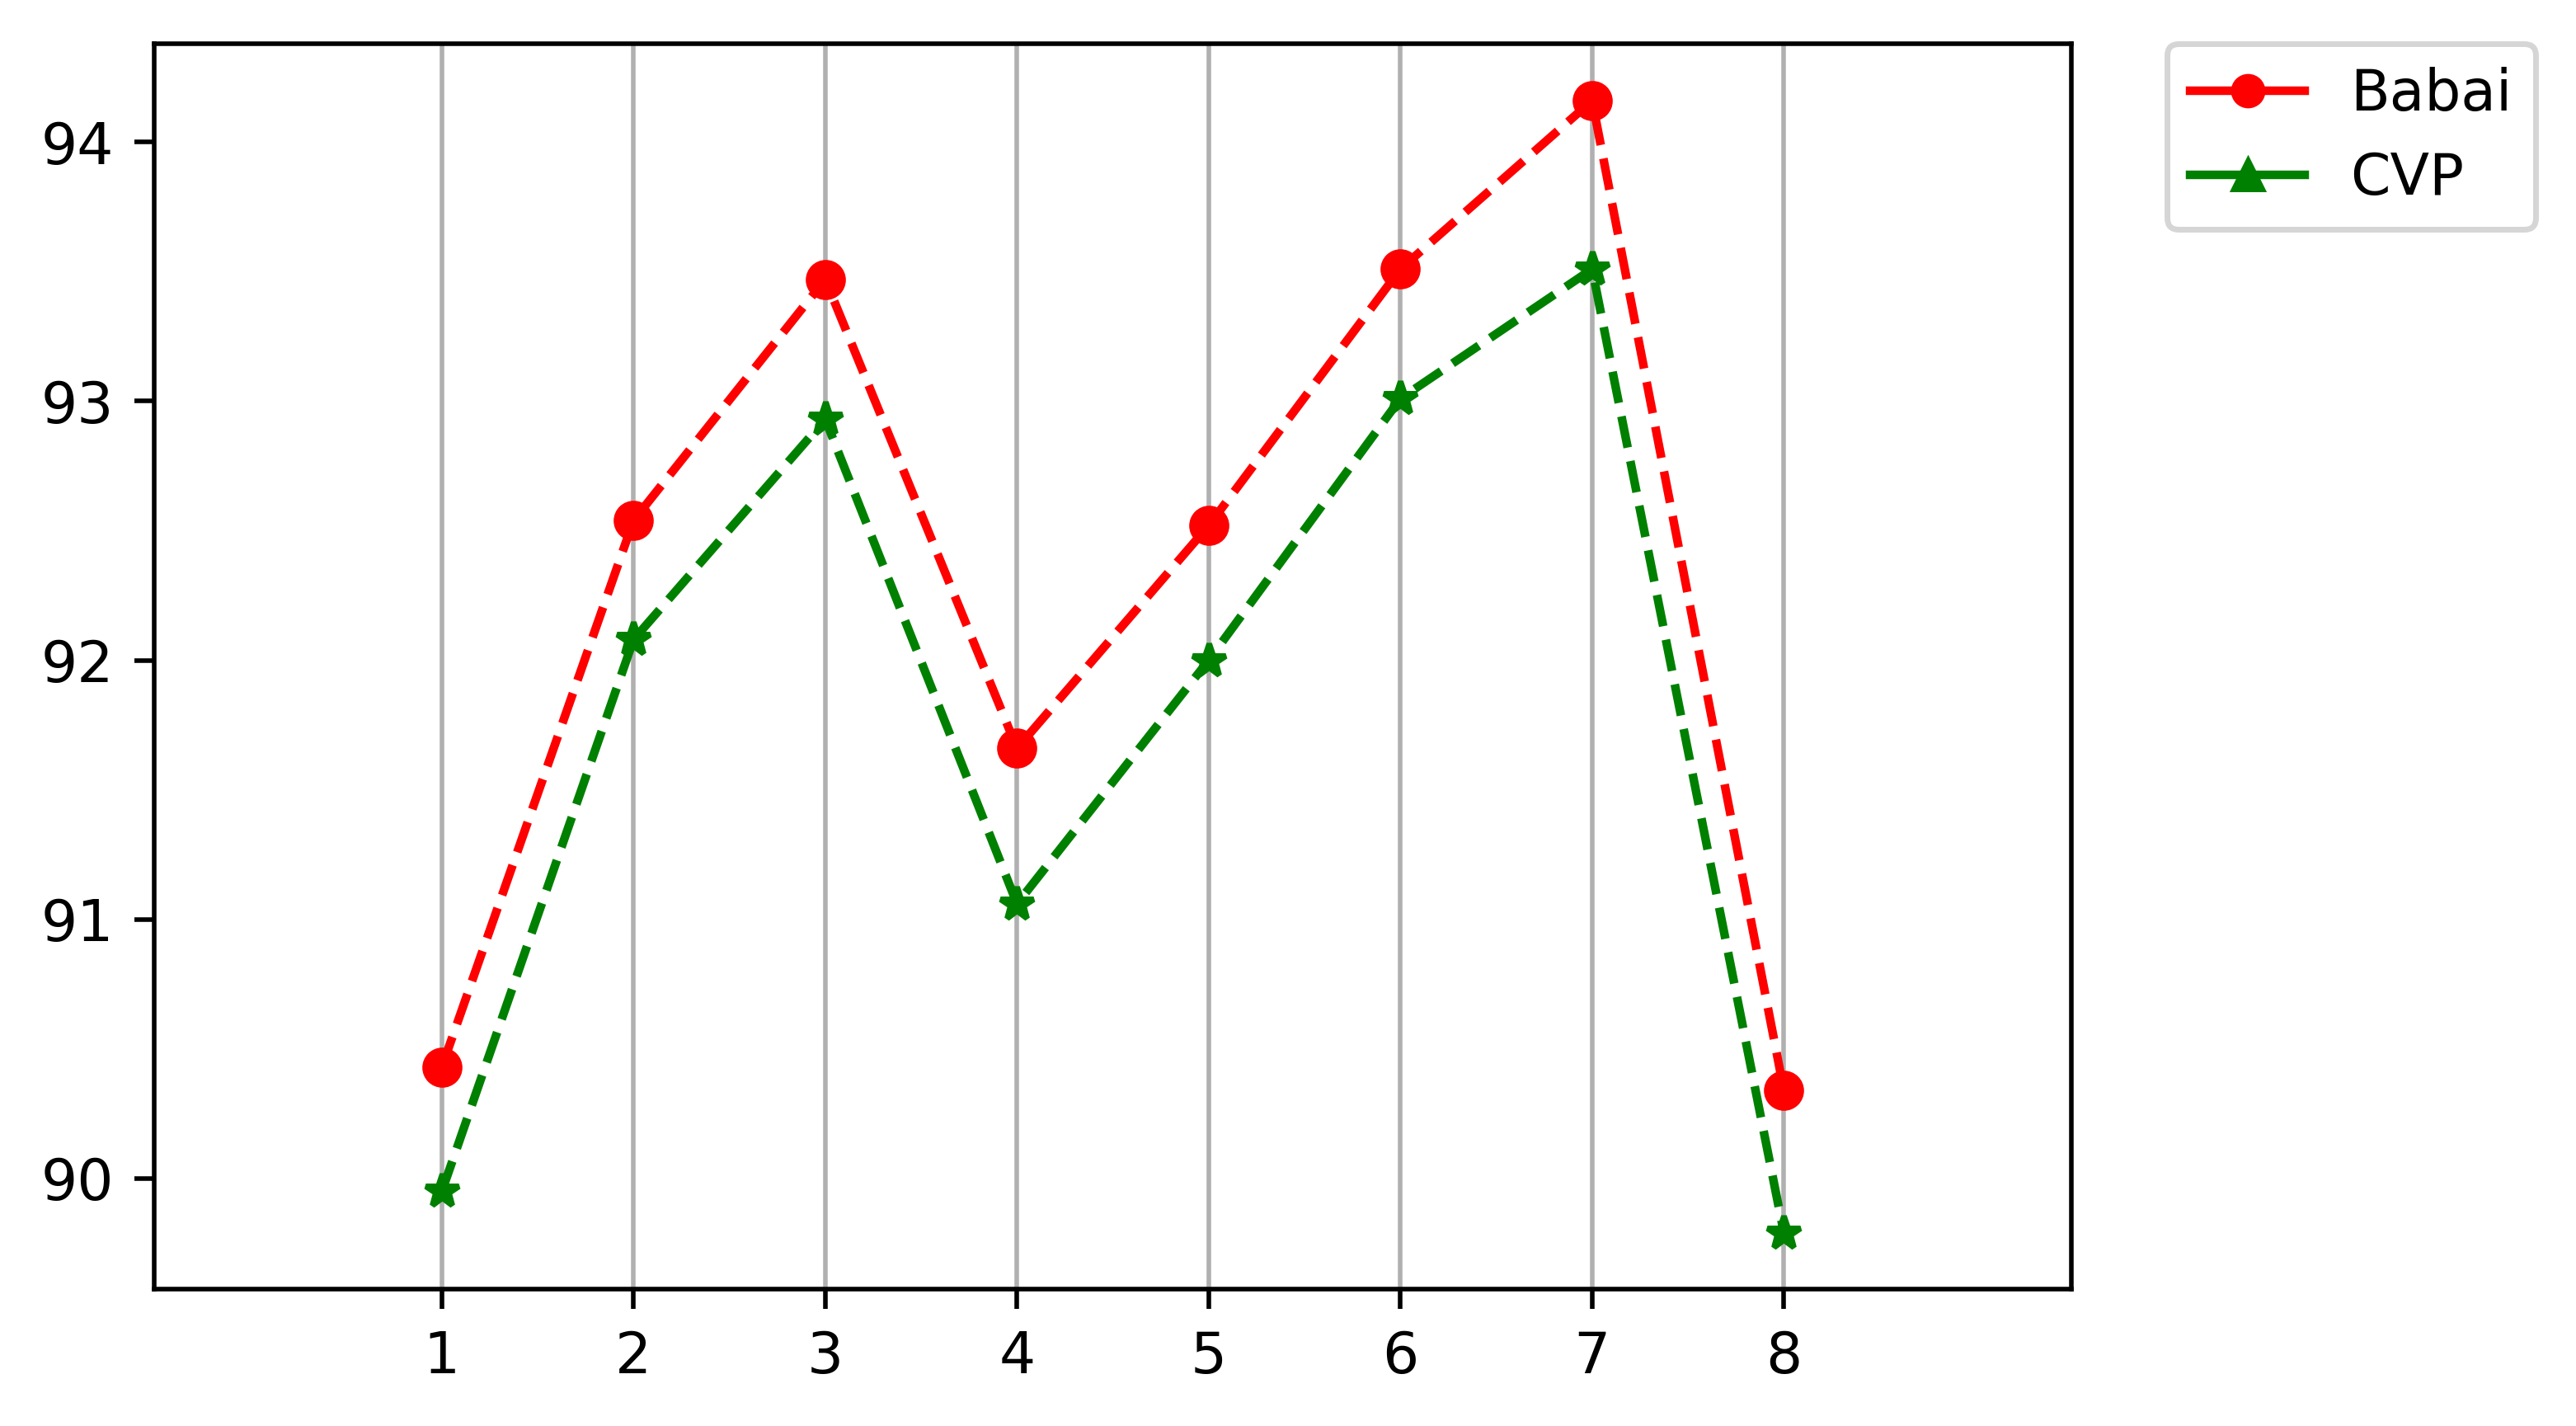
\includegraphics{1.png}}}
\caption{We use the matrix (\ref{vfk-matrix}) with $N=677$ and parameters $(P,q,k)=(6,70,10).$ We execute Babai and CVP (using the min-cut algorithm) with various target vectors of the form ${\bf t}\xleftarrow{\$} \{0,1\}^N \times \{-1000,...,1000\}^N.$ The $y-$axis contains $||{\bf x}-{\bf t}||,$ where ${\bf x}$ is either the output from CVP or Babai.}
\label{Fig.1}
\end{figure}

\begin{figure}[h!tb]
\centering
\rotatebox{0}{\scalebox{0.5}{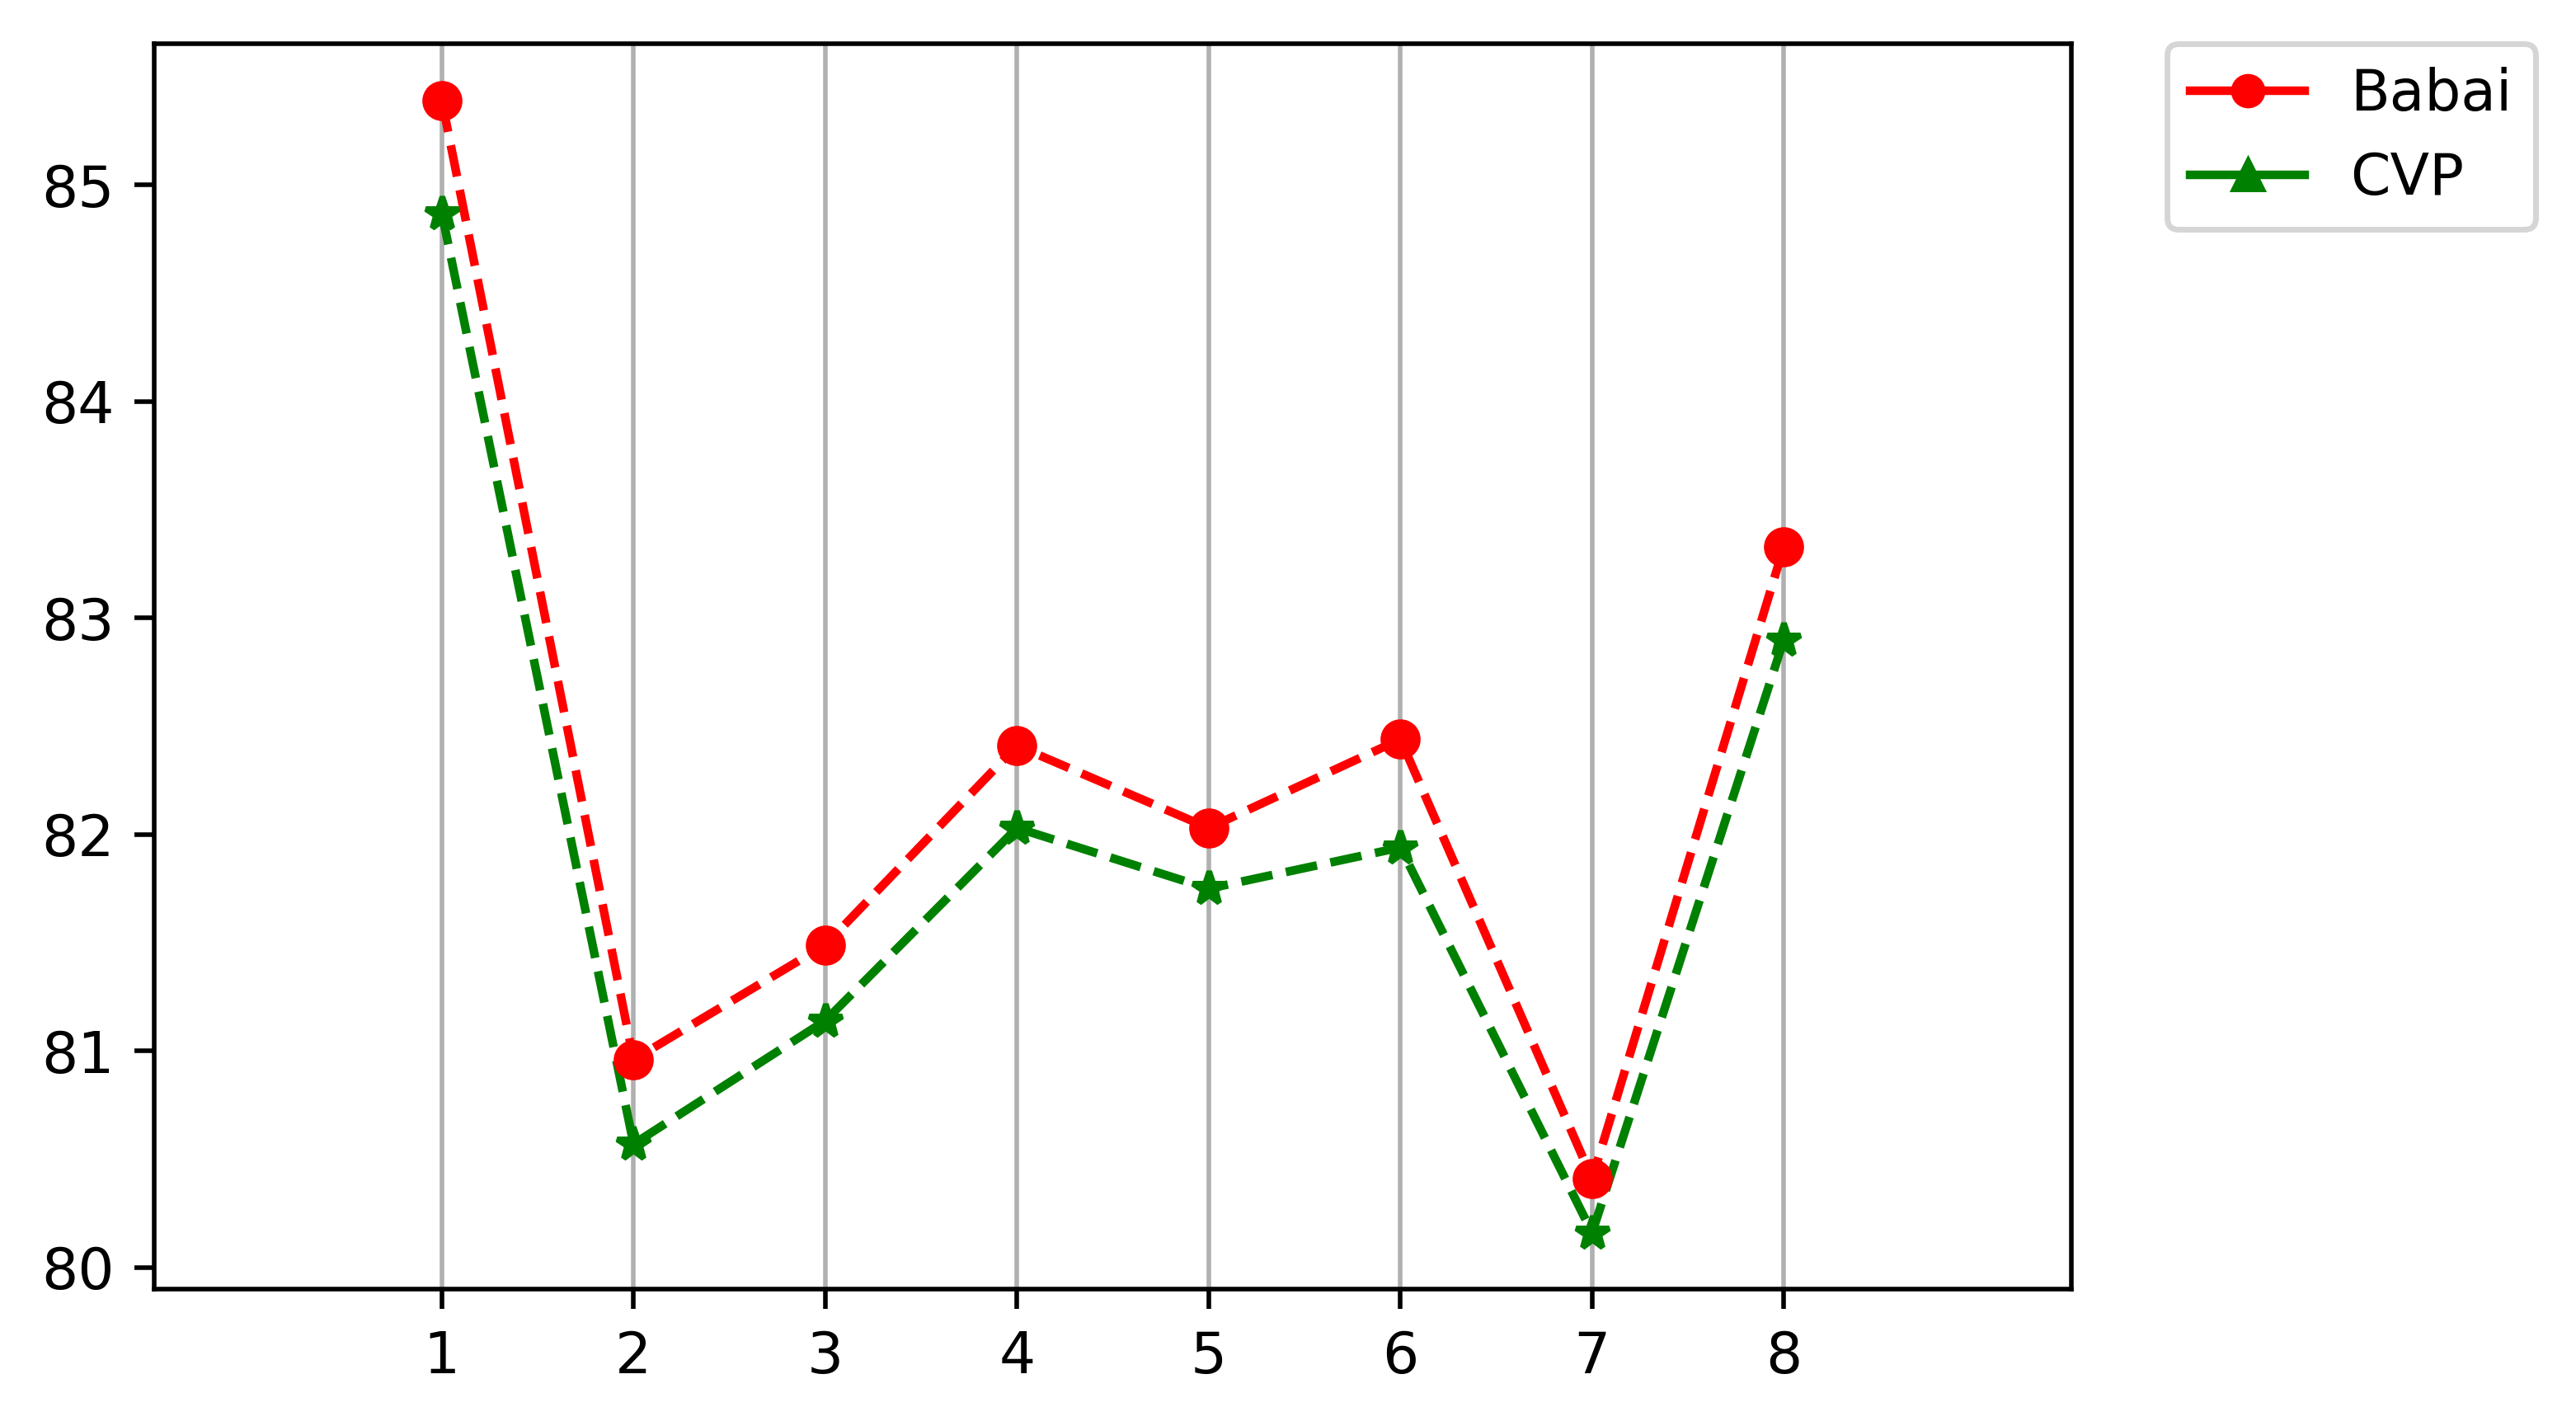
\includegraphics{2.png}}}
\caption{We fix the matrix (\ref{vfk-matrix}) with $N=557$ and parameters $(P,q,k)=(6,70,10).$  We execute Babai and CVP (using the min-cut algorithm) with various  target vectors of the form ${\bf t}\xleftarrow{\$} \{0,1\}^N \times \{-1000,...,1000\}^N.$ The $y-$axis contains $||{\bf x}-{\bf t}||,$ where ${\bf x}$ is either the output from CVP or Babai. The $x-$axis counts the number of experiments.}
\label{Fig.2}
\end{figure}

\begin{figure}[h!tb]
\centering
\rotatebox{0}{\scalebox{0.3}{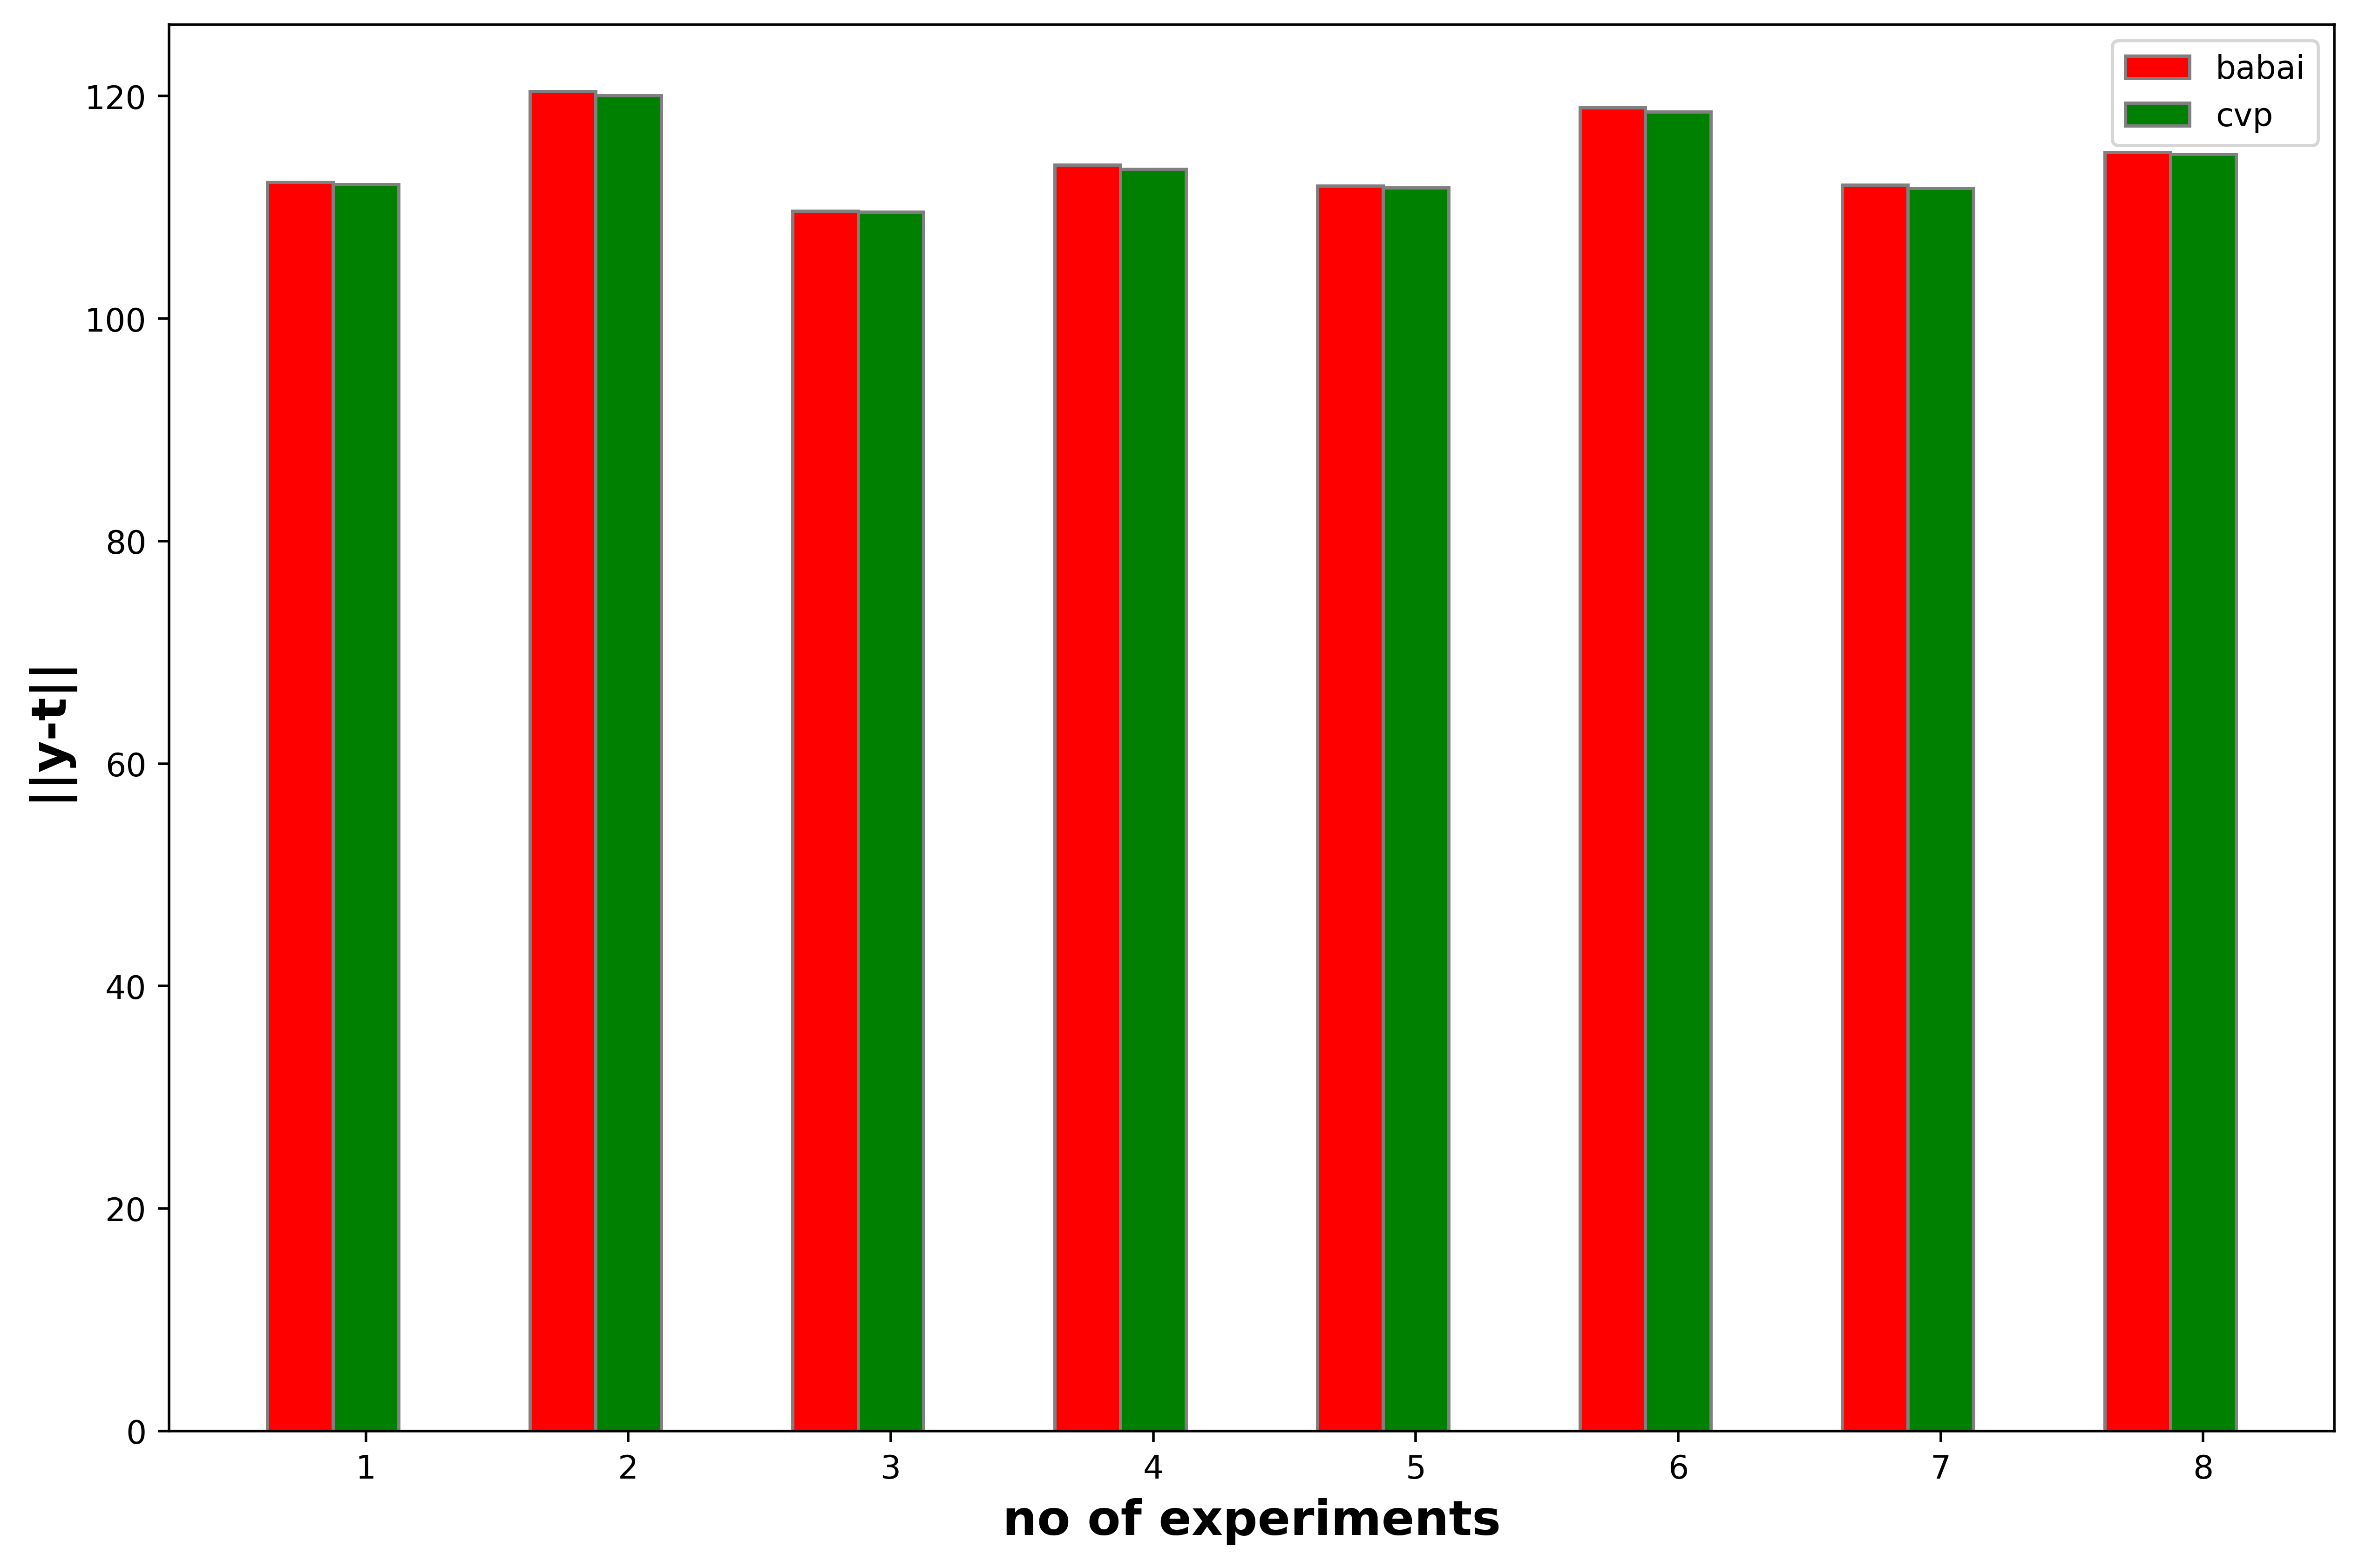
\includegraphics{3.png}}}
\caption{We fix the matrix (\ref{vfk-matrix}) with $N=239$ and parameters $(P,q,k)=(11,256,23).$  We execute Babai and CVP (using the min-cut algorithm) with various  target vectors of the form ${\bf t}\xleftarrow{\$} \{0,1\}^N \times \{-1000,...,1000\}^N.$ The $y-$axis contains $||{\bf y}-{\bf t}||,$ where ${\bf y}$ is either the output from CVP or Babai. The $x-$axis counts the number of experiments.}
\label{Fig.3}
\end{figure}

In all the experiments Babai's algorithm provided a larger vector. However, the distance between the two vectors, i.e. the one provided by CVP and the other provided by Babai, are very close.

\end{document}
\ \\
- We replace the approximate CVP-oracle (given by Babai)  with a CVP-oracle.
- We extend our attack to the other NTRU flavors such as NTRU-prime.\\
- Transferring the attack to VFK type lattices, it also improves the simplest Babai attack.
- In \texttt{ntruhps2048509} our method is proven better then Babai's attack in the same lattice.
- A non trivial connection of NTRU lattice with a VFK lattice is discovered.


